\renewcommand{\theequation}{\theenumi}
\begin{enumerate}[label=\arabic*.,ref=\thesubsection.\theenumi]
\numberwithin{equation}{enumi}
%
\item Solve
\begin{align}
\max_{\vec{x}} Z &= \myvec{4 & 1}\vec{x}
\\
s.t. \quad 
\myvec{
1 & 1
\\
3 & 1
}
\vec{x} &\preceq \myvec{50\\90}
\\
\vec{x} &\succeq \vec{0}
\end{align}
%
\solution The given problem can be expressed in general as
\begin{align}
\max_{\vec{x}} &\vec{c}^{T}\vec{x}
\\
s.t. \quad \vec{A}\vec{x} &\le \vec{b},
\\
\vec{x} &\succeq\vec{0}
\end{align}
%
where
\begin{align}
\vec{c} &= \myvec{4 \\ 1}
\\
\vec{A} &=
\myvec{
1 & 1
\\
3 & 1
}
\\
\vec{b}&=\myvec{50\\90}
%
\end{align}
%
and can be solved using {\em cvxpy} through the following code
\begin{lstlisting}
codes/line/lp_exam.py
\end{lstlisting}
%
to obtain
\begin{align}
\vec{x} = \myvec{30\\0}, Z = 120
\end{align}
%
%\begin{figure}[!ht]
%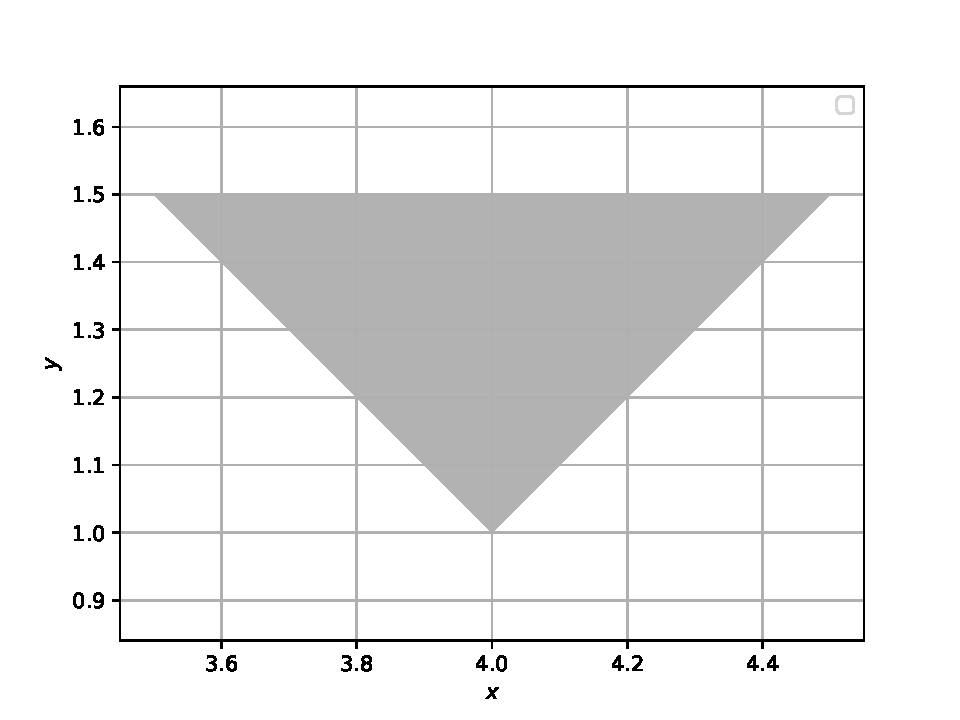
\includegraphics[width=\columnwidth]{./line/figs/line_ineq.eps}
%\caption{}
%\label{fig:line_ineq}
%\end{figure}
%

\item Solve
\begin{align}
\min_{\vec{x}} Z &= \myvec{3 & 9}\vec{x}
\\
s.t. \quad 
\myvec{
1 & 3
\\
-1 & -1
\\
1 & -1
}
\vec{x} &\preceq \myvec{60\\-10\\0}
\\
\vec{x} &\succeq \vec{0}
\label{eq:lp_exam_mult}
\end{align}
\solution The following code
\begin{lstlisting}
codes/line/lp_exam_mult.py
\end{lstlisting}
%
is used to obtain
\begin{align}
\vec{x} = \myvec{15\\15}, Z = 180
\end{align}


The region in \eqref{eq:lp_constr} is shown in Fig. \ref{}
\item Solve
\begin{align}
\min_{\vec{x}} Z &= \myvec{-50 & 20}\vec{x}
\\
s.t. \quad 
\myvec{
-2 & 1
\\
-3 & -1
\\
2 & -3
}
\vec{x} &\preceq \myvec{5\\-3\\12}
\\
\vec{x} &\succeq \vec{0}
\end{align}
%
\solution The following code 
\begin{lstlisting}
codes/line/lp_exam_nosol.py
\end{lstlisting}
%
shows that the given problem has no solution.
\item\textbf {(Diet problem)}: A dietician wishes to mix two types of foods in such a
way that vitamin contents of the mixture contain atleast 8 units of vitamin A and 10
units of vitamin C. Food ‘I’ contains 2 units/kg of vitamin A and 1 unit/kg of vitamin C.
Food ‘II’ contains 1 unit/kg of vitamin A and 2 units/kg of vitamin C. It costs
Rs 50 per kg to purchase Food ‘I’ and Rs 70 per kg to purchase Food ‘II’. Formulate
this problem as a linear programming problem to minimise the cost of such a mixture.\\
\item \textbf{(Allocation problem)} A cooperative society of farmers has 50 hectare
of land to grow two crops X and Y. The profit from crops X and Y per hectare are
estimated as Rs 10,500 and Rs 9,000 respectively. To control weeds, a liquid herbicide
has to be used for crops X and Y at rates of 20 litres and 10 litres per hectare. Further,
no more than 800 litres of herbicide should be used in order to protect fish and wild life
using a pond which collects drainage from this land. How much land should be allocated
to each crop so as to maximise the total profit of the society?\\
\item  \textbf{(Manufacturing problem)} A manufacturing company makes two models
A and B of a product. Each piece of Model A requires 9 labour hours for fabricating
and 1 labour hour for finishing. Each piece of Model B requires 12 labour hours for
fabricating and 3 labour hours for finishing. For fabricating and finishing, the maximum
labour hours available are 180 and 30 respectively. The company makes a profit of
Rs 8000 on each piece of model A and Rs 12000 on each piece of Model B. How many
pieces of Model A and Model B should be manufactured per week to realise a maximum
profit? What is the maximum profit per week?\\
\item \textbf {(Diet problem)} A dietician has to develop a special diet using two foods
P and Q. Each packet (containing 30 g) of food P contains 12 units of calcium, 4 units
of iron, 6 units of cholesterol and 6 units of vitamin A. Each packet of the same quantity
of food Q contains 3 units of calcium, 20 units of iron, 4 units of cholesterol and 3 units
of vitamin A. The diet requires atleast 240 units of calcium, atleast 460 units of iron and
at most 300 units of cholesterol. How many packets of each food should be used to
minimise the amount of vitamin A in the diet? What is the minimum amount of vitamin A?\\
\item \textbf{(Manufacturing problem)} A manufacturer has three machines I, II
and III installed in his factory. Machines I and II are capable of being operated for
at most 12 hours whereas machine III must be operated for atleast 5 hours a day. She
produces only two items M and N each requiring the use of all the three machines.
The number of hours required for producing 1 unit of each of M and N on the three
machines are given in the following table:\\

\begin{tabular}{|c|c|c|c|}
\hline
 \multicolumn{3}{|l}{\textbf{ Number of hours required on machines}}& \\ \cline{2-4}
\hline
\textbf {Items}&\textbf{I}&\textbf{II}&\textbf{III}\\
\hline
M&1&2&1\\
\hline
 N&2&1&1.25\\
 \hline 

\end{tabular}

She makes a profit of Rs 600 and Rs 400 on items M and N respectively. How many
of each item should she produce so as to maximise her profit assuming that she can sell
all the items that she produced? What will be the maximum profit?\\
\item \textbf{(Transportation problem)} There are two factories located one at
place P and the other at place Q. From these locations, a certain commodity is to be
delivered to each of the three depots situated at A, B and C. The weekly requirements
of the depots are respectively 5, 5 and 4 units of the commodity while the production
capacity of the factories at P and Q are respectively 8 and 6 units. The cost of transportation per unit is given below where A,B,C are cost in ruppes:\\
\begin{tabular}{|c|c|c|c|}
\hline
From/To & A & B & C\\
\hline
P & 160 & 100 & 150\\
\hline
Q & 100 &120 & 100\\
\hline
\end{tabular}\\
How many units should be transported from each factory to each depot in order that
the transportation cost is minimum. What will be the minimum transportation cost?\\





\end{enumerate}
%    \end{document}
    
